\label{sec::2_bg}
To generate dynamically balanced walking trajectories for humanoid robots and to let them navigate the environment autonomously, there are several posed challenges that we need to cover. As the logical starting point, in section \ref{sec::21_hw} - Humanoid Walking, we want to address the real-time generation of walking trajectories for humanoid robots first, and then think of ways to replace the human user by an artificial agent in the control loop (fig. \ref{fig::2_cl}). The generation of patterns in real-time becomes feasible by treating the robot's physics in a simplified way as those of an inverted pendulum (sec. \ref{sec::21_zmp}). The zero moment point of the linear inverted pendulum will, therefore, serve as the balance criteria for the solution of a sequentially quadratic problem (sec. \ref{sec::22_nmpc}).  Resulting positions and orientations for the center of mass and the feet will then be interpolated (sec. \ref{sec::23_it}) and be passed as constraints to the inverse kinematics (sec. \ref{sec::241_fk}) so to transform them into joint angles that can be sent to the humanoid's motor controllers.
\begin{figure}[h!]
	\centering
	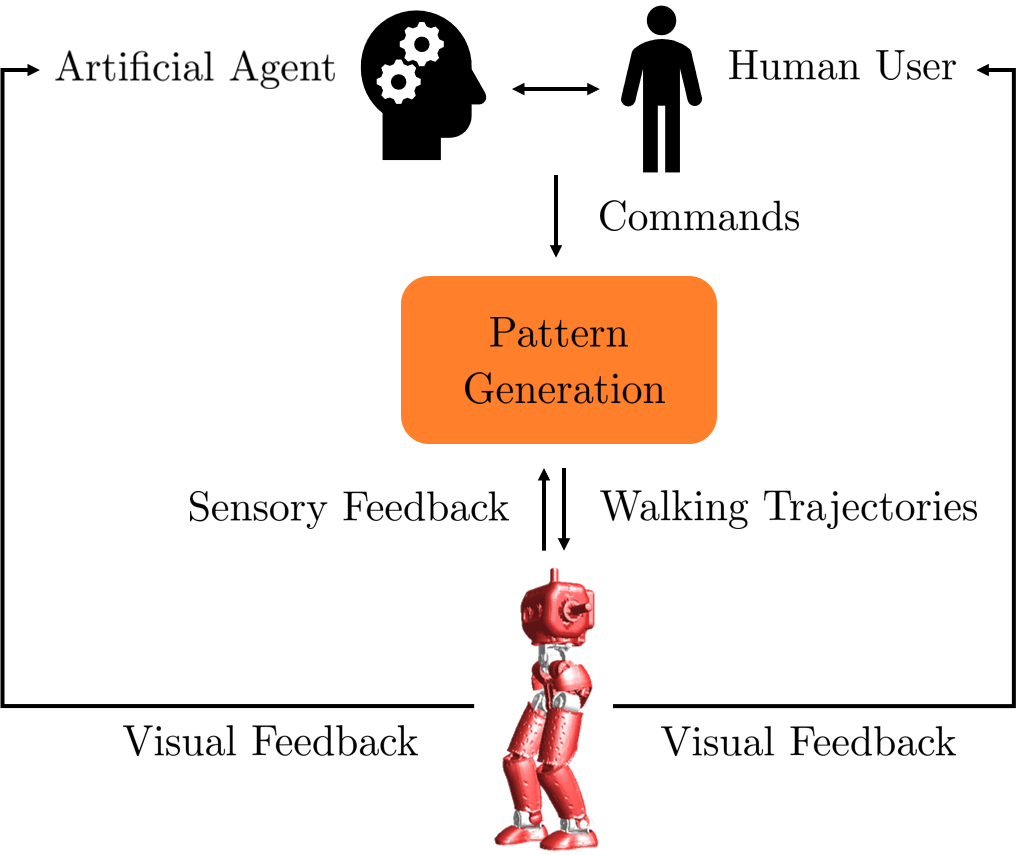
\includegraphics[scale=.5]{chapters/06_implementing_an_autonomous_walking_pattern_generator/img/control_loop.png}
	\caption{Simplified version of the proposed control loop to navigate the robot with either a human user or an artificial agent. The commands will be given in the form of linear velocities $v_x$, and $v_y$, along the x-, and the y-axis, as well as an angular velocity $\omega_z$ about the z-axis of the robot's coordinates system.}
	\label{fig::2_cl}
\end{figure}
\\
To close the control loop and to steer the robot towards desired goals, whilst avoiding obstacles, requires some high-level command that arises from visual feedback. As discussed in section \ref{sec::1_in} - Introduction, there are several ways to achieve this, among them human users. Of particular interest to us are novel methods that evolved from the toolbox of machine learning techniques, as they decrease the computational cost into nonexistence. Let alone this fact enables us to run them onboard on lightweight hardware with low energy usage, which is critical in the domain of humanoid robots. Center to these new methods will be neural nets that we will train on solving the task of autonomous navigation in two different ways. One of which clones the behavior of a human user (sec. \ref{sec::51_bc}), whereas the second presented method (sec. \ref{sec::32_rl}) explores policies and tries to find solutions on its own.
\\\\
\textbf{Note:} Within the following chapters, there will always be made references to the actual implementation of the presented concepts, which shall enable future readers to bridge the gap between theory and application.